C++通过异常机制提供了通知和处理错误的框架。因为有些错误发生在设备上,或者在设备上启动工作时,所以异构编程还需要对错误级别进行管理。这些错误通常与主程序不相关,因此不能与C++异常处理机制集成。为了解决这个问题,需要有其他机制使异步错误易于管理和控制。\par

图5-1展示了程序的两个部分:(1)主机代码运行的顺序,以及执行和提交工作任务图(2)的异步执行和函数或对其他设备操作,对主程序的运行的依赖性。例子使用parallel\_for执行内核函数,并作为任务图的一部分异步执行,其他的操作会在第3、4和8章中再进行讨论。\par

\hspace*{\fill} \par %插入空行
图5-1 分离主程序和内核任务
\begin{center}
	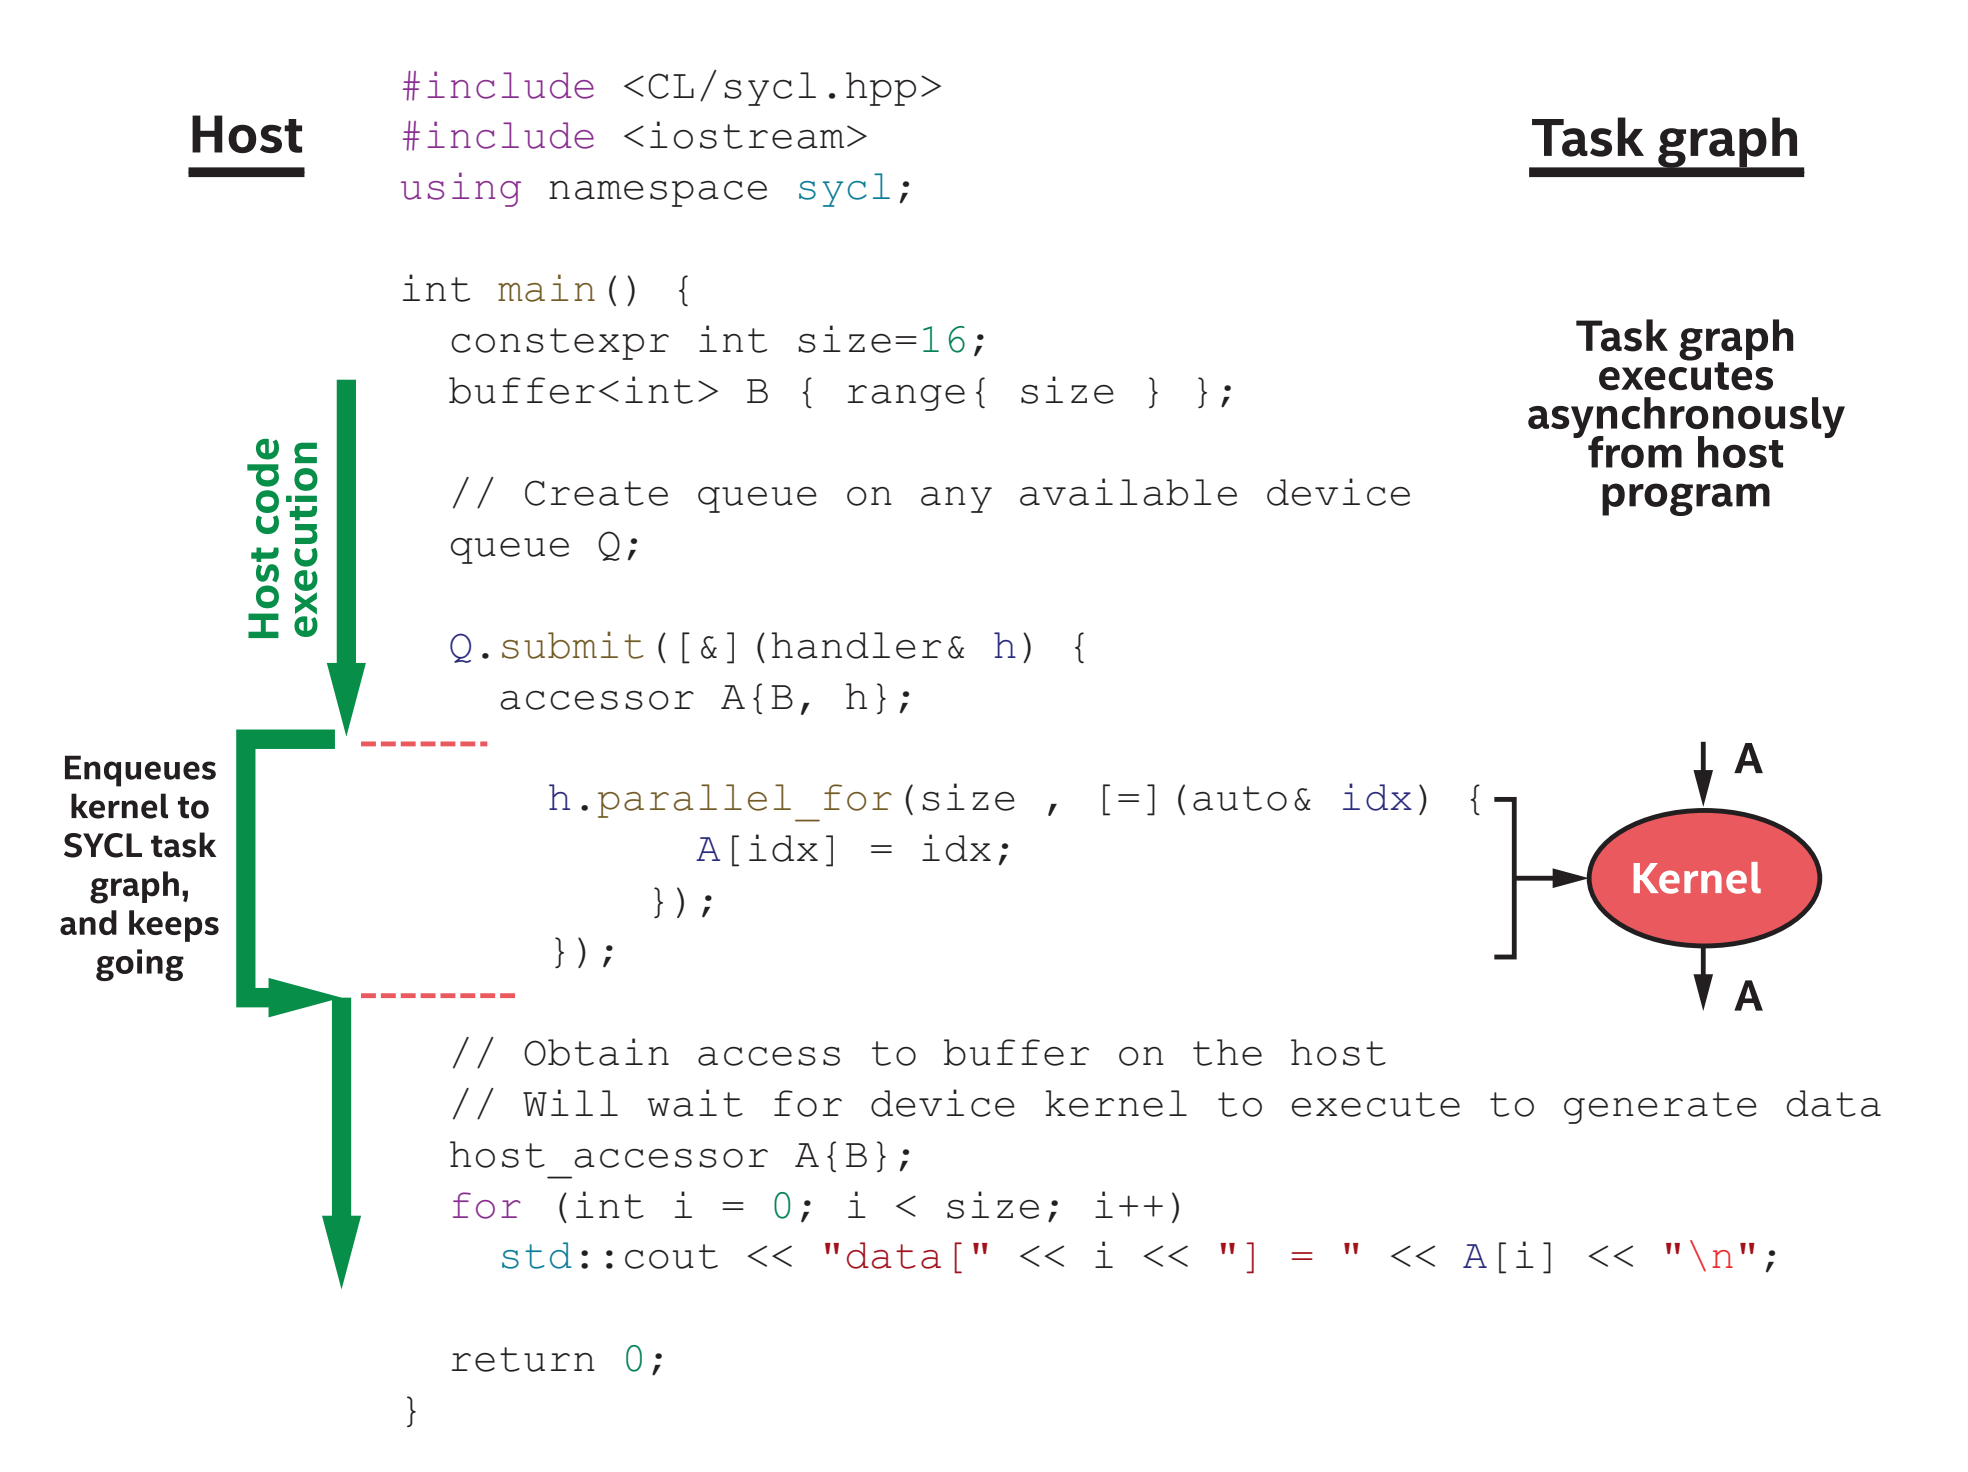
\includegraphics[width=1.0\textwidth]{content/chapter-5/images/2}
\end{center}

理解图5-1中左边和右边(主机和任务图)之间的区别,是理解同步和异步错误区别的关键。\par

主程序执行某个操作(如API调用或对象构造函数),在检测到错误条件时,会发生同步错误。可以在图左侧的指令完成前检测到,并且可以立即将错误抛出。可以在图的左侧使用try-catch来包装指令,在try块结束(从而捕获)前检测到try中操作的错误。C++异常机制就是为了处理这些错误而设计的。\par

当图5-1右侧出现异步错误时,只有在执行中的操作才会检测到错误。当检测到异步错误时,主程序通常会继续执行,所以无法使用try-catch来捕获这些错误。不过,有异步异常处理框架可以来处理这些错误。\par










